\myChapter{Généralité sur la sécurité des systèmes d'information}{}\label{chapGénéralité}

%\myMinitoc{Profondeur de la minitoc (section|subsection|subsubsection)}{Titre de la minitoc}
\myMiniToc{section}{Table des matières}

%\mySection{Introduction}{}\label{sectionIntroduction}

Dans ce chapitre nous fournirons la base terminologique nécessaire à la compréhension de ce travail. Nous présenterons une brève introduction à la sécurité des systèmes d'information et présenterons le concept de contrôle d'accès.

\mySection{Sécurité des systèmes d'information}{}\label{sectionSécuritéSI}

\mySubSection{Définition de la sécurité}{}\label{sectionSécurité}
Le terme sécurité correspond au mot anglais « Security » et traduit la capacité du système informatique à résister à des agressions externes physiques (incendie, inondation, bombes.) ou logiques (erreurs de saisie, intrusions, piratages, logique malicieuse.). C'est généralement le sens choisi par les spécialistes de l'audit de sécurité, lorsqu'ils doivent, pour une entreprise donnée, évaluer les risques liés à l'informatique.Les ITSEC \cite{jahl91} définissent la sécurité comme la combinaison de trois propriétés : la confidentialité, l'intégrité et la disponibilité de l'information. L'information représente en plus des données et des programmes, les traitements effectués sur les informations. Ici, la sécurité, implique d'empêcher la réalisation d'opérations illégitimes contribuant à mettre en défaut les propriétés de confidentialité, d'intégrité et de disponibilité, mais aussi de garantir la possibilité de réaliser les opérations légitimes dans le système. Assurer la sécurité du système revient à assurer que les propriétés retenues sont vérifiées, et garantir la non-occurrence de défaillances vis-à-vis de ces propriétés \cite{theseBenoit}.

\mySubSection{Confidentialité}{}\label{sectionConfidentialité}
  La confidentialité est la propriété d'une information à ne pas être révélée à des utilisateurs non autorisés à la connaître. Le système informatique doit empêcher les utilisateurs de lire une information confidentielle (sauf s'ils y sont autorisés), et d'empêcher les utilisateurs autorisés à lire une information et de la divulguer à d'autres utilisateurs (sauf autorisation). Assurer la confidentialité d'un système est une tâche complexe. Il faut analyser tous les chemins qu'une information particulière peut prendre dans le système pour s'assurer qu'ils sont sécurisés. Il faut également prendre en compte les connaissances qu'un ou plusieurs utilisateurs peuvent déduire à partir des informations acquises. Il faut donc contrôler non seulement les informations présentes dans le système, mais aussi les liens logiques qui peuvent les relier entre elles ou à des informations publiques. Les attaques contre la confidentialité consistent à essayer d'obtenir des informations qui doivent être protégées selon la politique de sécurité, en dépit des moyens de protection et des règles de sécurité \cite{theseBenoit}.

\mySubSection{Intégrité}{}\label{sectionIntégrité}

L'intégrité est la propriété d'une information à ne pas être altérée. Le système informatique doit \cite{theseBenoit} :
\begin{itemize}
\item Empêcher une modification de l'information par des utilisateurs non autorisés ou une modification incorrecte par des utilisateurs autorisés; 
\item Faire en sorte qu'aucun utilisateur ne puisse empêcher la modification légitime de l'information. Par exemple, empêcher la mise à jour périodique d'un compteur de temps constituerait une atteinte à l'intégrité; 
\item Assurer que toute modification de donnée est approuvée et que chaque programme se comporte de manière correcte (conformément aux fonctions qu'il est censé remplir, y compris dans ses interactions avec les autres processus.); 
\item Assurer qu'aucune information ne peut être modifiée par des intermédiaires, que cette altération soit intentionnelle (par exemple, un utilisateur intervient pour modifier une communication entre deux autres utilisateurs.) ou accidentelle (une donnée modifiée lorsqu'elle est communiquée via un support de communication non-fiable).
\end{itemize}

\mySubSection{Disponibilité}{}\label{sectionDisponibilité}
La disponibilité est la propriété d'une information d'être accessible lorsqu'un utilisateur autorisé en a besoin. Le système informatique doit \cite{theseBenoit}:
\begin{itemize}

\item Fournir l'accès à l'information pour que les utilisateurs autorisés puissent la lire ou la modifier ; 
\item Faire en sorte qu'aucun utilisateur ne puisse empêcher les utilisateurs autorisés d'accéder à l'information.
\end{itemize}

\hspace*{0.5cm} Dans le souci de garantir la non-violation de ces propriétés de sécurité, plusieurs techniques de sécurité à l'instar du contrôle d'accès ont été proposé dans la section suivante nous présenterons la notion de contrôle d'accès.

\mySection{Contrôle d'accès}{}\label{sectionContrôle}

\mySubSection{Définition du contrôle d'accès}{}\label{sectionDéfinition}

Le contrôle d'accès est une technique de sécurité qui vise à limiter ce qu'un utilisateur ou les programmes s'exécutant au nom de cet utilisateur sont autorisés à faire dans le système. Ainsi le contrôle d'accès permet d'empêcher toute activité susceptible de conduit à une violation de la sécurité. Son but est de limiter les actions ou les opérations qu'un utilisateur légitime du système informatique peut effectuer. Le modèle de base de toutes les politiques de contrôle d'accès est montré sur la figure \ref{figAc}:
\begin{figure}[h!]
    \centering
		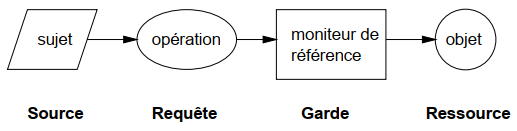
\includegraphics[scale=0.7]{chap1/images/Ac.png}
    \caption{Modèle de base du contrôle d'accès \cite{jensen99}}
	 \label{figAc}
\end{figure}
\\
\hspace*{0.5 cm} La figure montre un sujet qui souhaite faire une opération sur un objet. Le système transforme l'opération en une requête qu'il passe au moniteur de référence (qui est un médiateur incontournable dans toutes les relations entre sujets et objets. Le moniteur de référence est responsable de l'autorisation de l'accès à un objet par un sujet.) qui contrôle l'accès aux ressources. Si le sujet est autorisé à accéder à l'objet selon la politique de sécurité en vigueur, l'accès à l'objet va être accordé et l'opération peut se dérouler normalement \cite{jensen99}.

\mySubSection{Le contrôle d'accès et les autres services}{}\label{sectionAccès}
 Dans un système informatique, le contrôle d'accès repose sur d'autres services de sécurité et coexiste avec eux. 
\begin{itemize}

\item \textbf{Contrôle d'accès et l'administrateur de sécurité:} Le contrôle d'accès vise à limiter l'activité des utilisateurs légitimes. Il est appliqué par le moniteur de référence qui sert d'intermédiaire à chaque tentative d'accès d'un utilisateur (ou un programme s'exécutant au nom de cet utilisateur) aux objets du système. Le moniteur de référence consulte une base de données d'autorisations afin de déterminer si un utilisateur tentant d'effectuer une opération est réellement autorisé à effectuer cette opération. Les autorisations de cette base de données sont gérées et administrées par l'administrateur de sécurité. L'administrateur définit ces autorisations sur la base de la politique de sécurité de l'organisation. Les utilisateurs peuvent également modifier une partie de cette base de données des autorisations, par exemple, pour définir les autorisations pour leurs fichiers personnels\cite{sandhu94}. 


\item \textbf{Le contrôle d'accès et l'authentification:} Il est important de faire une distinction entre l'authentification et le contrôle d'accès. L'établissement correct de l'identité de l'utilisateur relève de la responsabilité de l'authentification. Le contrôle d'accès suppose que l'authentification  de l'utilisateur a été vérifiée avec succès avant l'application du contrôle d'accès via le moniteur de référence. L'efficacité du contrôle d'accès repose sur une identification correcte de l'utilisateur et sur l'exactitude des autorisations accordées au moniteur de référence \cite{sandhu94}.


\item \textbf{contrôle d'accès et l'audit:} Il est important de comprendre que le contrôle d'accès n'est pas une solution complète pour sécuriser le système. Il doit être couplé à l'audit. L'audit permet de surveiller et d'enregistrer les activités pertinentes dans le système. Les contrôles d'audit concernent une analyse à posteriori de toutes les demandes et activités des utilisateurs dans le système. L'audit nécessite l'enregistrement de toutes les demandes et activités des utilisateurs pour une analyse ultérieure. Les contrôles d'audit sont utiles à la fois comme moyen de dissuasion et comme moyen d'analyser le comportement des utilisateurs dans l'utilisation du système afin de découvrir d'éventuelles tentatives ou violation réelles.  En outre, l'audit peut être utilisé pour déterminer les éventuelles failles du système de sécurité. En fin il est essentiel pour garantir que les utilisateurs autorisés n'abusent pas de leurs privilèges. En d'autres termes, pour les tenir responsables de leurs actions \cite{sandhu94}.
\end{itemize} 

\begin{figure}[h!]
    \centering
		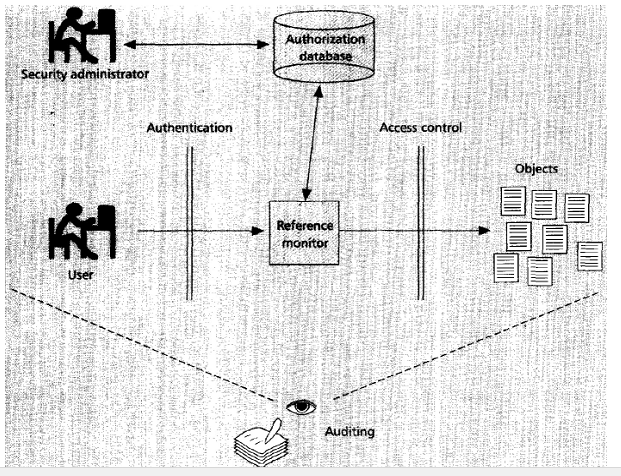
\includegraphics[scale=0.7]{chap1/images/controle.png}
    \caption{Contrôle d'accès et autres services de sécurité \cite{sandhu94}}
	 \label{figcontrole}
\end{figure}

\mySubSection{Politique de sécurité}{}\label{sectionPolitiqueSécurité}
Dans un système informatique, l'autorisation a pour but de ne permettre que les actions légitimes, d'empêcher qu'un utilisateur puisse exécuter des opérations qui ne lui sont pas permises. Pour définir quelles sont les opérations autorisées et celles qui sont interdites, il faut établir une politique de sécurité ou « doctrine de sécurité » \cite{theseBenoit}. Dans les systèmes de contrôle d'accès, une distinction est généralement faite entre les politiques et les mécanismes de sécurité. Les politiques sont des directives de haut niveau qui déterminent comment les accès sont contrôlés et les décisions d'accès déterminées. Alors que les mécanismes sont des fonctions logicielles et matérielles de bas niveau qui peuvent être configurées pour mettre en œuvre une politique. Au fil des années, il a été développé par des chercheurs et pratiquants de la sécurité des mécanismes de sécurité qui sont indépendants des politiques de sécurité. Les politiques de contrôle d'accès ne sont pas nécessairement exclusives. Différents politiques peuvent être combinés pour fournir un système de protection plus adapté. Lorsque les politiques sont combinées, seule l'intersection de leur accès est autorisée. Une telle combinaison de politique est relativement simple tant qu'il n'y a pas de conflits entre une politique qui affirme qu'un accès particulier doit être autorisé et une autre qui l'interdit. Ces conflits sont conciliés par des négociations à un niveau de gestion approprié \cite{sandhu94}.

\mySubSection{Conclusion}{}\label{sectionConclusion}
%\\
 En conclusion, il était question pour nous dans ce chapitre de présenter les concepts de base de notre travail.

%\myCleanStarChapterEnd